\chapter{Characterization Methods}
\label{ch:characterization}
\thispagestyle{empty}

%%%%%%%%%%%%%%%%%%%%%%%%%%%%%%%%%%%%%%%%%%%%%%%%%%%
%%%%%%%%%%%%%%%%%%%%%%%%%%%%%%%%%%%%%%%%%%%%%%%%%%%
%%%%%%%%%%%%%%%%%%%%%%%%%%%%%%%%%%%%%%%%%%%%%%%%%%%

\section{Imaging Techniques}

A variety of imaging methods were used to visually inspect the samples at a variety of length scales. The two main techniques that proved invaluable for this aspect of the project were scanning electron microscopy (SEM) as well as atomic force microscopy (AFM). 

%%%%%%%

\subsection{Scanning Electron Microscopy}

Scanning electron microscopy is a widely used technique for imaging nanostructures. 

\lipsum


%%%%%%%
	
\subsection{Atomic Force Microscopy}
	
\lipsum

%%%%%%%%%%%%%%%%%%%%%%%%%%%%%%%%%%%%%%%%%%%%%%%%%%%
%%%%%%%%%%%%%%%%%%%%%%%%%%%%%%%%%%%%%%%%%%%%%%%%%%%
%%%%%%%%%%%%%%%%%%%%%%%%%%%%%%%%%%%%%%%%%%%%%%%%%%%

\section{Compositional Analysis}

%%%%%%%

\subsection{Energy-Dispersive X-Ray Spectroscopy}

\lipsum

%%%%%%%

\subsection{X-Ray Fluorescence Spectroscopy}

\lipsum

%%%%%%%

\subsection{Rutherford Backscattering Spectroscopy}

\lipsum

%%%%%%%%%%%%%%%%%%%%%%%%%%%%%%%%%%%%%%%%%%%%%%%%%%%
%%%%%%%%%%%%%%%%%%%%%%%%%%%%%%%%%%%%%%%%%%%%%%%%%%%
%%%%%%%%%%%%%%%%%%%%%%%%%%%%%%%%%%%%%%%%%%%%%%%%%%%

\section{Thin Film Characterization}


%%%%%%%
	
\subsection{Variable Angle Spectroscopic Ellipsometry}

Ellipsometry is a powerful non-destructive optical technique that allows for the determination of a large number of properties of complex thin film structures. The basic tenet of ellipsometry relies on the analysis of the change in polarization state of a reflected light beam after interaction with the sample. The incident beam is generally linearly polarized, but upon reflection becomes elliptically polarized due to a phase shift in the components of the beam in the s- and p-plane, as well as a change in their relative amplitudes. The phase shift is correlated to the ellipsometric parameter $\Delta$, while the amplitude change is given by $\tan\Psi$ ($\Psi$ is the angle between the s-plane and the major axis of the ellipse). The last major parameter is the incident angle, denoted by $\Phi$. A schematic diagram illustrating these parameters can be seen in figure~\ref{fig:ellipsometry}. 

\begin{figure}[htbp]
   \centering
   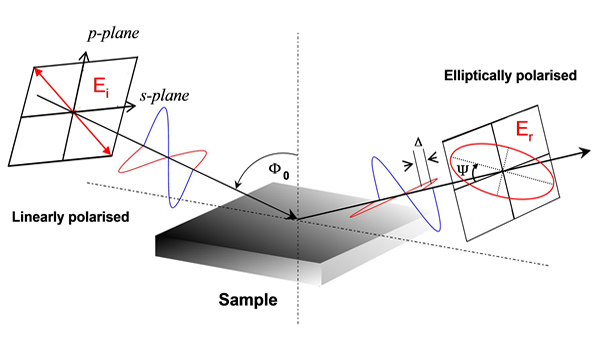
\includegraphics[width=\linewidth]{./figures/characterization/ellipsometryDiagram_simple} 
   \caption[Ellipsometric Beam Path and Modeling Parameters]{Schematic of the beam path during an %
   					ellipsometric measurement, \\ critical parameters are indicated}
   \label{fig:ellipsometry}
\end{figure}

From these parameters, one can directly determine the ratio between the reflectance in the p-plane ($r_{p}$) and the reflectance in the s-plane ($r_{s}$) from the fundamental ellipsometric relation (eqn.~\ref{eq:ellipsometry}).  Once this relationship is known, the Fresnel equations (eqn.~\ref{eq:fresnel}) can be used to numerically determine the value of the complex index of refraction at the specific wavelength of the incoming beam. The complex index of refraction (eqn.~\ref{eq:complexindex}) describes the nominal index of refraction but additionally includes an imaginary term to describe absorption of light in the material (commonly referred to as the extinction coefficient, $\kappa$).  

\begin{equation}
 \label{eq:ellipsometry}
 \displaystyle
	\rho = \frac{r_{p}}{r_{s}} = \tan(\Psi)e^{i\Delta}
\end{equation}

\begin{subequations}
\label{eq:fresnel}
\begin{align}
	r_{p} &= \frac{\tilde{n}_{1}\sqrt{1- \left(\frac{\tilde{n}_{1}}{\tilde{n}_{2}}\sin\Phi\right)} - \tilde{n}_{2}\cos\Phi}{\tilde{n}_{1}\sqrt{1- \left(\frac{\tilde{n}_{1}}{\tilde{n}_{2}}\sin\Phi\right)} + \tilde{n}_{2}\cos\Phi} \\
        	r_{s} &= \frac{\tilde{n}_{1}\cos\Phi - \tilde{n}_{2}\sqrt{1- \left(\frac{\tilde{n}_{1}}{n_{2}}\sin\Phi\right)}}{\tilde{n}_{1}\cos\Phi + \tilde{n}_{2}\sqrt{1- \left(\frac{\tilde{n}_{1}}{\tilde{n}_{2}}\sin\Phi\right)}}
\end{align}
\end{subequations}

\begin{equation}
 \label{eq:complexindex}
 \displaystyle
	\tilde{n} = n + i\kappa
\end{equation}

This type of analysis is sufficient for thick, isotropic samples without any surface layers (e.g. surface oxides or adsorbed gases), and can directly provide the value of $\tilde{n}$. However, once layers are stacked upon one another, the system becomes very difficult to analyze directly due to interference effects between the layers. It becomes necessary to use modeling techniques to determine the correct values of $\tilde{n}$ and thickness ($t$) for each layer. 

The power of ellipsometry as a high-resolution optical analysis technique stems from the use of phase and polarization changes. This allows the analysis to overcome the diffraction limit, and can be accurate down to angstroms. Properly modeling the system is critical for this analysis to be as precise as possible. Thus, there have been refinements of the ellipsometric method to greatly increase the amount of experimental data points, allowing the overall system to be over-determined and thus letting all of the systems parameters to be calculated. 
	
Variable angle spectroscopic ellipsometry (VASE) is one of these variants. Spectroscopic ellipsometry differs from single-wavelength ellipsometry by utilizing a broad-band light source as opposed to a monochromatic source. By performing ellipsometric analysis at each of the wavelengths, one can determine the wavelength (and thus photon-energy) dependence of $n$ and $\kappa$. This not only helps to improve data analysis (as it can generally be safely assumed that the values of $n$ and $\kappa$ are smooth functions of $\lambda$), but allows for the determination of many other properties of the material. Of specific importance is the complex dielectric function ($\tilde{\epsilon}$), which is related to $\tilde{n}$ by the relation shown in equation~\ref{eq:dielectricfunction}. Knowing this function can allow for determination of electronic properties such as the bandgap energy, the absorption coefficient, amongst others. Finally, by obtaining spectra at a number of different incident angles, one directly provides additional data points across the entire wavelength spectrum. Even a small number of additional angles can quickly provide sufficient data points for the system to be over determined. 

\begin{equation}
 \label{eq:dielectricfunction}
 \displaystyle
	\tilde{\epsilon} = \epsilon_{1} + i\epsilon_{2} = \tilde{n}^{2}
\end{equation}

During this project, a VASE M-2000U system (figure~\ref{fig:M2000_image}) built by J.A. Woollam, inc. was used to collect all of the ellipsometric data. In addition, data analysis was performed using the WVASE32 package also provided by J.A. Woollam. The system utilizes a rotating compensator and a CCD detector to greatly decrease data collection time by collecting data across the entire spectrum simultaneously.  More information on this system is available on J.A. Woollam, inc.'s webpage.\cite{woollam-web}

\begin{figure}[htbp]
   \centering
   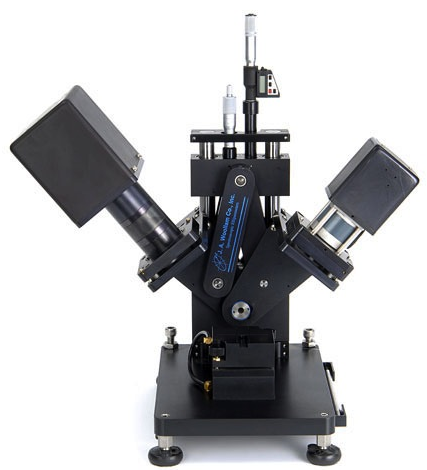
\includegraphics[width=0.33\linewidth]{./figures/characterization/M2000_ellipsometer_image.png} 
   \caption[J.A. Woollam M-2000U Ellipsometer]{Photograph of the J.A. Woollam M-2000U variable \\%
   									angle spectroscopic ellipsometer (VASE)}
   \label{fig:M2000_image}
\end{figure}


%%%%%%%%%%%%%%%%%%%%%%%%%%%%%%%%%%%%%%%%%%%%%%%%%%%
%%%%%%%%%%%%%%%%%%%%%%%%%%%%%%%%%%%%%%%%%%%%%%%%%%%
%%%%%%%%%%%%%%%%%%%%%%%%%%%%%%%%%%%%%%%%%%%%%%%%%%%
	
\section{Phase Identification}

%%%%%%%

\subsection{X-Ray Diffraction}

\lipsum	

%%%%%%%

\subsection{Grazing Incidence X-Ray Diffraction}

\lipsum

%%%%%%%%%%%%%%%%%%%%%%%%%%%%%%%%%%%%%%%%%%%%%%%%%%%
%%%%%%%%%%%%%%%%%%%%%%%%%%%%%%%%%%%%%%%%%%%%%%%%%%%
%%%%%%%%%%%%%%%%%%%%%%%%%%%%%%%%%%%%%%%%%%%%%%%%%%%

\section{Chemical Analysis}

%%%%%%%

\subsection{Thermogravimetric Analysis}

Thermogravimetric analysis (TGA) is a very useful tool when attempting to determine the viability of a precursor in an ALD process. It allows for estimation of vaporization rate at various temperature rates as well as indications of chemical breakdown (i.e. thermalization) which would negate the precursor's usefulness. 

At its core, TGA is a measurement of mass loss as a function of temperature or time. A small sample (1--10 mg) of material is placed in a microgram balance pan and suspended inside a furnace. The furnace is then heated at a specified rate while the sample mass is carefully monitored. For the experiments used in this study (evaluation of thermal vaporization and thermal degradation) it is important to ensure that the testing environment is inert. This is accomplished by using a platinum pan in the microgram balance and constantly purging the furnace with a small flow of dry nitrogen gas. The heating rate can be varied according to a pre-determined program to provide more information at various individual temperatures. 

This technique was used to evaluate various precursor candidates for the lead oxide half of the \PTO deposition procedure. A detailed discussion of TGA procedures and the investigated chemicals can be found in subsequent chapters (\ref{chap:TA-methods}). 

\begin{figure}[htbp] %%%%%%%%% maybe have subfigure for both TA systems?
   \centering
   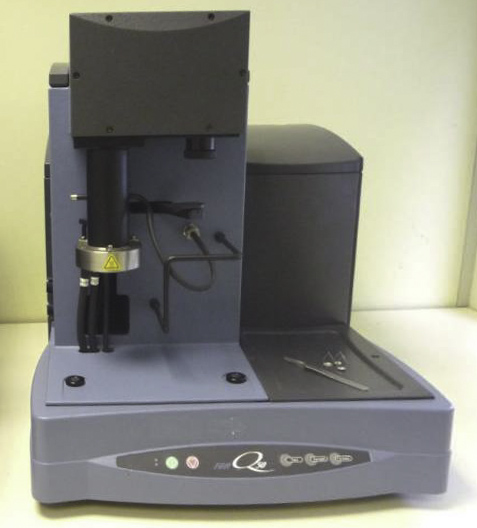
\includegraphics[width=0.5\linewidth]{./figures/characterization/Q50-TGA} 
   \caption[T.A. Instruments, inc. Q50 TGA System]%
   		{Photograph of the T.A. Instruments, inc. \\%
		 Q50 TGA system used during this study}
   \label{fig:Q50_image}
\end{figure}

%%%%%%%

\subsection{Differential Scanning Calorimetry}
	
\lipsum
	
	
	
	
	
	